%! TEX program = xelatex
\documentclass[UTF8,a4paper,12pt,fontset=fandol]{ctexart}

% ============================================================
% 2026 年全国大学生数学建模竞赛论文模板（电子版）
% 编译器：XeLaTeX
% 官方硬性要求：A4；四周页边距至少 2.5 cm；第一页为摘要；
% 不要目录；正文不超过 30 页；正文和附录不得出现身份信息。
% ============================================================

\usepackage[top=2.5cm,bottom=2.5cm,left=2.5cm,right=2.5cm]{geometry}
\usepackage{amsmath,amssymb,bm}
\usepackage{booktabs,tabularx,multirow,longtable,array}
\usepackage{graphicx,float,subcaption}
\usepackage{enumitem}
\usepackage{xcolor}
\usepackage{listings}
\usepackage{url}
\usepackage[hidelinks]{hyperref}
\usepackage{appendix}

\graphicspath{{figures/}}
\setlength{\parindent}{2em}
\setlength{\parskip}{0pt}
\linespread{1.25}
\pagestyle{plain}

\ctexset{
  section={format=\zihao{4}\bfseries,beforeskip=1.2ex,afterskip=0.8ex},
  subsection={format=\zihao{-4}\bfseries,beforeskip=1ex,afterskip=0.6ex},
  subsubsection={format=\zihao{-4}\bfseries,beforeskip=0.8ex,afterskip=0.4ex}
}

\captionsetup{font=small,labelsep=quad}
\setlist{nosep,leftmargin=2em}

\lstset{
  basicstyle=\small\ttfamily,
  numbers=left,
  numberstyle=\tiny\color{gray},
  frame=single,
  breaklines=true,
  showstringspaces=false,
  keywordstyle=\color{blue!70!black},
  commentstyle=\color{green!45!black},
  stringstyle=\color{purple}
}

\begin{document}
\pagenumbering{arabic}
\setcounter{page}{1}

% ======================== 摘要专用页 ========================
\begin{center}
  {\zihao{3}\bfseries 论文题目}
\end{center}

\begin{center}
  {\zihao{4}\bfseries 摘\quad 要}
\end{center}

这里填写摘要。建议按照“研究对象—四个问题的方法—主要结果—模型检验—结论”组织。
摘要要给出关键数值结果，不要只写背景和建模过程。题目、摘要和关键词原则上不得超过一页。

\vspace{0.8em}
\noindent\textbf{关键词：}关键词一；关键词二；关键词三；关键词四

% 2026 年官方规范明确要求：正文前不要目录。
\newpage

% =========================== 正文 ===========================
\section{问题重述}
\subsection{问题背景}
用自己的语言概括现实背景，不要大段照抄赛题。

\subsection{问题要求}
分别概括各问的目标、已知条件、约束和所需输出。

\section{问题分析}
\subsection{问题一分析}
说明研究对象、关键变量、建模思路和预期结果。

\subsection{问题二分析}
说明该问与前一问的联系，以及分组、预测或优化思路。

\subsection{问题三分析}
说明需要增加的因素、约束条件和验证方法。

\subsection{问题四分析}
说明标签定义、判定规则和评价指标。

\section{模型假设}
\begin{enumerate}
  \item 假设一，并说明其合理性；
  \item 假设二，并说明忽略该因素可能带来的影响；
  \item 假设三。
\end{enumerate}

\section{符号说明}
\begin{table}[H]
  \centering
  \caption{主要符号说明}
  \begin{tabularx}{\textwidth}{cXc}
    \toprule
    符号 & 含义 & 单位 \\
    \midrule
    $x$ & 示例变量，请替换 & -- \\
    $y$ & 示例响应变量，请替换 & -- \\
    \bottomrule
  \end{tabularx}
  \label{tab:symbols}
\end{table}

\section{数据预处理}
说明数据来源、缺失值、异常值、重复记录、变量单位和衍生变量。所有处理应能由附录中的程序复现。

\section{问题一的模型建立与求解}

\subsection{表面风化与玻璃类型的关系}

为分析不同玻璃类型与表面风化之间的关系，本文将玻璃类型和
表面风化状态分别作为两个分类变量，首先计算不同玻璃类型的
风化比例，并建立列联表进行独立性检验。

统计结果表明，40件铅钡玻璃中有28件发生表面风化，样本风化率为
$70.00\%$；18件高钾玻璃中有6件发生表面风化，样本风化率为$33.33\%$。两类玻璃的样本风化率存在较为明显的差异，具体结果如图~\ref{fig:weathering-type} 所示。

\begin{figure}[htbp]
  \centering
  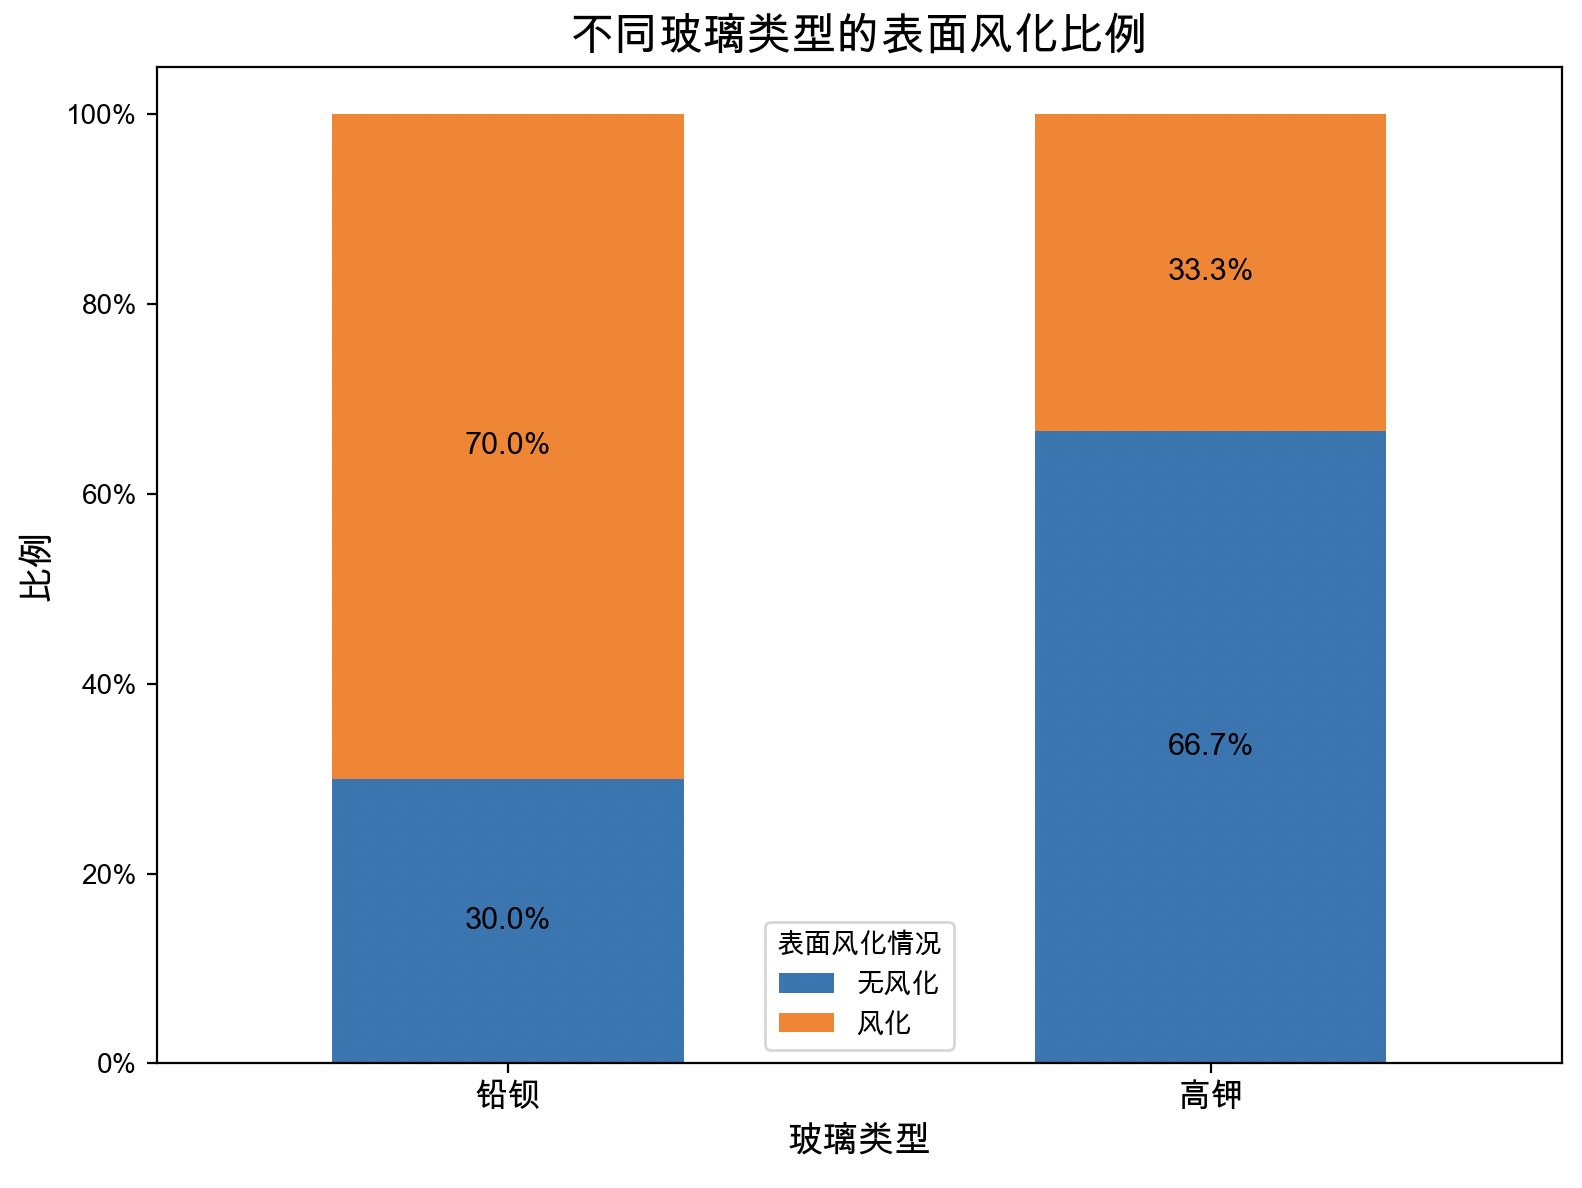
\includegraphics[width=0.72\textwidth]{weathering_by_type.png}
  \caption{不同玻璃类型的表面风化比例}
  \label{fig:weathering-type}
\end{figure}

为进一步判断玻璃类型与表面风化是否存在统计关联，建立如下假设：

\[
H_0:\text{玻璃类型与表面风化相互独立},
\]

\[
H_1:\text{玻璃类型与表面风化存在关联}.
\]

采用 Pearson 卡方独立性检验，得到

\[
\chi^2=6.880,\qquad p=0.0087<0.05.
\]

因此，在 $5\%$ 的显著性水平下拒绝原假设，认为玻璃类型与
表面风化之间存在显著关联。为检验结论的稳健性，进一步采用 Fisher 精确检验作为补充检验，
得到 $p=0.0113<0.05$，其结论与 Pearson 卡方检验一致。


同时，Cramér's $V$ 为

\[
V=0.344,
\]

说明玻璃类型与表面风化之间具有一定程度的关联。结合描述性统计
结果可知，在现有样本中，铅钡玻璃表现出比高钾玻璃更高的表面
风化倾向。

\subsection{表面风化与颜色的关系}

\subsubsection{数据处理与描述性统计}

为分析玻璃文物颜色与表面风化之间的关系，本文将颜色和表面风化状态
视为两个分类变量，并建立列联表进行关联分析。附件表单~1 共包含 58 件
玻璃文物，其中 4 件文物的颜色记录为“未知”。由于“未知”表示颜色信息
缺失，并非实际颜色类别，故将其排除，最终得到 54 件有效样本，包含
8 种颜色。各颜色文物的风化情况如表~\ref{tab:color-weathering} 所示。

\begin{table}[htbp]
    \centering
    \caption{不同颜色玻璃文物的表面风化情况}
    \label{tab:color-weathering}
    \begin{tabular}{ccccc}
        \toprule
        颜色 & 样本量 & 风化数量 & 无风化数量 & 风化率 \\
        \midrule
        黑   & 2  & 2  & 0 & $100.00\%$ \\
        浅蓝 & 20 & 12 & 8 & $60.00\%$  \\
        蓝绿 & 15 & 9  & 6 & $60.00\%$  \\
        深绿 & 7  & 4  & 3 & $57.14\%$  \\
        紫   & 4  & 2  & 2 & $50.00\%$  \\
        浅绿 & 3  & 1  & 2 & $33.33\%$  \\
        深蓝 & 2  & 0  & 2 & $0.00\%$   \\
        绿   & 1  & 0  & 1 & $0.00\%$   \\
        \bottomrule
    \end{tabular}
\end{table}

由表~\ref{tab:color-weathering} 可知，不同颜色文物在样本中呈现出不同的
风化比例。其中，浅蓝和蓝绿文物的风化率均为 $60.00\%$，深绿文物为
$57.14\%$，紫色文物为 $50.00\%$。黑色样本全部发生风化，而深蓝和
绿色样本均未发生风化。

然而，各颜色类别的样本量明显不均衡。浅蓝和蓝绿分别包含 20 件和
15 件文物，而黑、深蓝和绿色分别仅有 2 件、2 件和 1 件。因此，小样本
类别中出现的 $0\%$ 或 $100\%$ 风化率可能主要受到随机波动影响，不能
仅依据样本风化率判断颜色与表面风化之间是否存在稳定关联。

\subsubsection{Pearson 卡方检验及其适用性检查}

由于颜色和表面风化状态均为分类变量，首先采用 Pearson 卡方独立性检验
判断二者是否存在总体关联。建立假设
\begin{equation}
    \begin{aligned}
        H_0 &: \text{颜色与表面风化相互独立},\\
        H_1 &: \text{颜色与表面风化存在关联}.
    \end{aligned}
\end{equation}

在 $H_0$ 成立的条件下，第 $i$ 种颜色与第 $j$ 种风化状态组合的期望频数为
\begin{equation}
    E_{ij}=\frac{n_{i\cdot}n_{\cdot j}}{n},
\end{equation}
相应的 Pearson 卡方统计量为
\begin{equation}
    \chi^2=\sum_{i=1}^{r}\sum_{j=1}^{c}
    \frac{(O_{ij}-E_{ij})^2}{E_{ij}},
\end{equation}
其中，$O_{ij}$ 为实际观测频数，$n_{i\cdot}$ 与 $n_{\cdot j}$ 分别为
对应行总数和列总数，$n$ 为总样本量。

计算得到
\begin{equation}
    \chi^2=6.2871,\qquad df=7,\qquad p=0.5066.
\end{equation}
普通渐近结果未达到 $0.05$ 的显著性水平。但是，在 16 个列联表单元格中，
有 12 个单元格的期望频数小于 5，占比为 $75.00\%$；其中 4 个单元格的
期望频数小于 1，最小期望频数仅为 $0.4444$。因此，该列联表具有明显
稀疏性，不满足 Pearson 卡方检验的大样本近似条件，不能将其渐近 $p$ 值
作为最终判断依据。

\subsubsection{Monte Carlo 检验与效应量}

针对稀疏列联表，本文在保持列联表行、列边际结构的条件下进行 $100000$
次随机模拟，构造原假设成立时卡方统计量的经验分布，并以模拟结果中不小于
实际统计量的比例估计显著性概率。Monte Carlo 检验得到
\begin{equation}
    p_{\mathrm{MC}}=0.5809>0.05.
\end{equation}
因此，在 $5\%$ 的显著性水平下不能拒绝原假设。就颜色这一整体分类变量
而言，现有 54 件有效样本尚未提供充分证据表明颜色与表面风化存在显著
总体关联。

为描述样本中颜色与风化状态的关联程度，进一步计算 Cram\'{e}r's $V$
效应量：
\begin{equation}
    V=\sqrt{\frac{\chi^2}{n\min(r-1,c-1)}}=0.3412.
\end{equation}
该数值表明样本中存在一定程度的表观结构差异，但效应量不能代替显著性
检验。由于 Monte Carlo 检验未通过，且部分颜色类别样本量极小，当前
观察到的样本差异尚不能推广为稳定的总体关联。

\subsubsection{玻璃类型的潜在混杂作用}

前文已经证明玻璃类型与表面风化存在显著关联：铅钡玻璃的样本风化率为
$70.00\%$，高钾玻璃为 $33.33\%$，Pearson 卡方检验得到
$p=0.0087<0.05$。与此同时，各颜色对应的玻璃类型构成并不均衡。
例如，黑色、紫色、浅绿色和绿色样本全部属于铅钡玻璃；浅蓝色样本中
铅钡玻璃占 $80.00\%$，深绿色样本中铅钡玻璃占 $85.71\%$；蓝绿色
样本中高钾玻璃则占 $80.00\%$。

分层观察也可以发现这种影响。浅蓝色铅钡玻璃共有 16 件，其中 12 件
风化，样本风化率为 $75.00\%$；浅蓝色高钾玻璃共有 4 件，均未风化。
蓝绿色铅钡玻璃共有 3 件，均发生风化；蓝绿色高钾玻璃共有 12 件，其中
6 件风化，样本风化率为 $50.00\%$。由于分层后的部分样本量仍然较小，
上述比例只能作为描述性证据，但足以说明颜色所呈现的部分风化率差异
可能受到玻璃类型构成差异的影响。

\subsubsection{结论}

综合描述性统计、稀疏列联表的 Monte Carlo 检验和混杂因素分析可知：
不同颜色文物在当前样本中的风化率存在差异，但整体检验结果为
$p_{\mathrm{MC}}=0.5809>0.05$，尚无充分统计证据认定颜色与表面风化
存在显著总体关联。该结论不等同于“每一种具体颜色都与风化无关”，而是
表示在当前样本量和类别结构下，尚不能证明颜色具有独立、稳定的风化效应。
考虑到玻璃类型本身与风化显著相关，且颜色与玻璃类型的构成高度不均衡，
部分表观颜色差异可能主要反映玻璃类型的潜在混杂作用。

\subsection{不同玻璃类型风化组与无风化组的化学成分差异}

\subsubsection{数据分组与预处理}

附件表单~2 共包含 69 个化学成分采样点。按照题目给出的有效性标准，
将成分总和不在 $85\%\sim105\%$ 范围内的 15 号和 17 号采样点剔除，
最终保留 67 个有效采样点。对于未检出的化学成分，以 0 记录；随后将每个
有效采样点的 14 种化学成分归一化至总和为 $100\%$，以消除不同样本总量
差异对组间比较的影响。

为避免玻璃类型的混杂作用，本文不直接混合高钾玻璃与铅钡玻璃，而是在
两类玻璃内部，按照采样点实际风化状态分别构造风化组与无风化组。高钾
玻璃包括 12 个无风化采样点和 6 个风化采样点；铅钡玻璃包括 23 个无风化
采样点和 26 个风化采样点。

\subsubsection{统计方法的选择}

部分化学成分含有较多零值，分布具有明显偏态；同时，高钾玻璃风化组仅有
6 个样本，难以保证独立样本 $t$ 检验所要求的近似正态性。因此，本文首先
利用箱线图比较两组数据的中位数、四分位距和离散程度，再采用对总体分布
形式要求较低的 Mann--Whitney $U$ 检验，对同一玻璃类型下风化组与无风化
组的成分分布进行比较。

对于每一种化学成分，建立假设
\begin{equation}
    \begin{aligned}
        H_0 &: \text{风化组与无风化组的总体分布不存在系统差异},\\
        H_1 &: \text{风化组与无风化组的总体分布存在系统差异}.
    \end{aligned}
\end{equation}

设风化组和无风化组样本量分别为 $n_1$ 和 $n_2$，以风化组对应的
$U$ 统计量计算秩二列效应量
\begin{equation}
    r_{\mathrm{rb}}=\frac{2U}{n_1n_2}-1.
\end{equation}
其中，$r_{\mathrm{rb}}>0$ 表示风化组的取值整体偏高，
$r_{\mathrm{rb}}<0$ 表示风化组的取值整体偏低，
$|r_{\mathrm{rb}}|$ 越大表示两组分布分离程度越明显。

两类玻璃各检验 14 种化学成分，共进行 $m=28$ 次比较。为控制多重检验
产生的假阳性，本文对原始 $p$ 值实施 Benjamini--Hochberg 校正。将原始
$p$ 值从小到大排列为 $p_{(1)},\ldots,p_{(m)}$，相应校正值为
\begin{equation}
    q_{(i)}=\min_{j\geq i}\left\{\frac{m}{j}p_{(j)}\right\},
\end{equation}
并以 $q<0.05$ 作为差异显著的判断标准。

\subsubsection{箱线图分析}

高钾玻璃中，风化组二氧化硅的整体分布明显高于无风化组；氧化钾、
氧化镁、氧化铝和五氧化二磷的分布则整体偏低，如图~\ref{fig:q1b-high-k}
所示。二氧化硅和氧化钾的两组分离最为明显。氧化钙、氧化铁和氧化铅
也呈现下降趋势，但两组样本仍有一定重叠。

\begin{figure}[H]
    \centering
    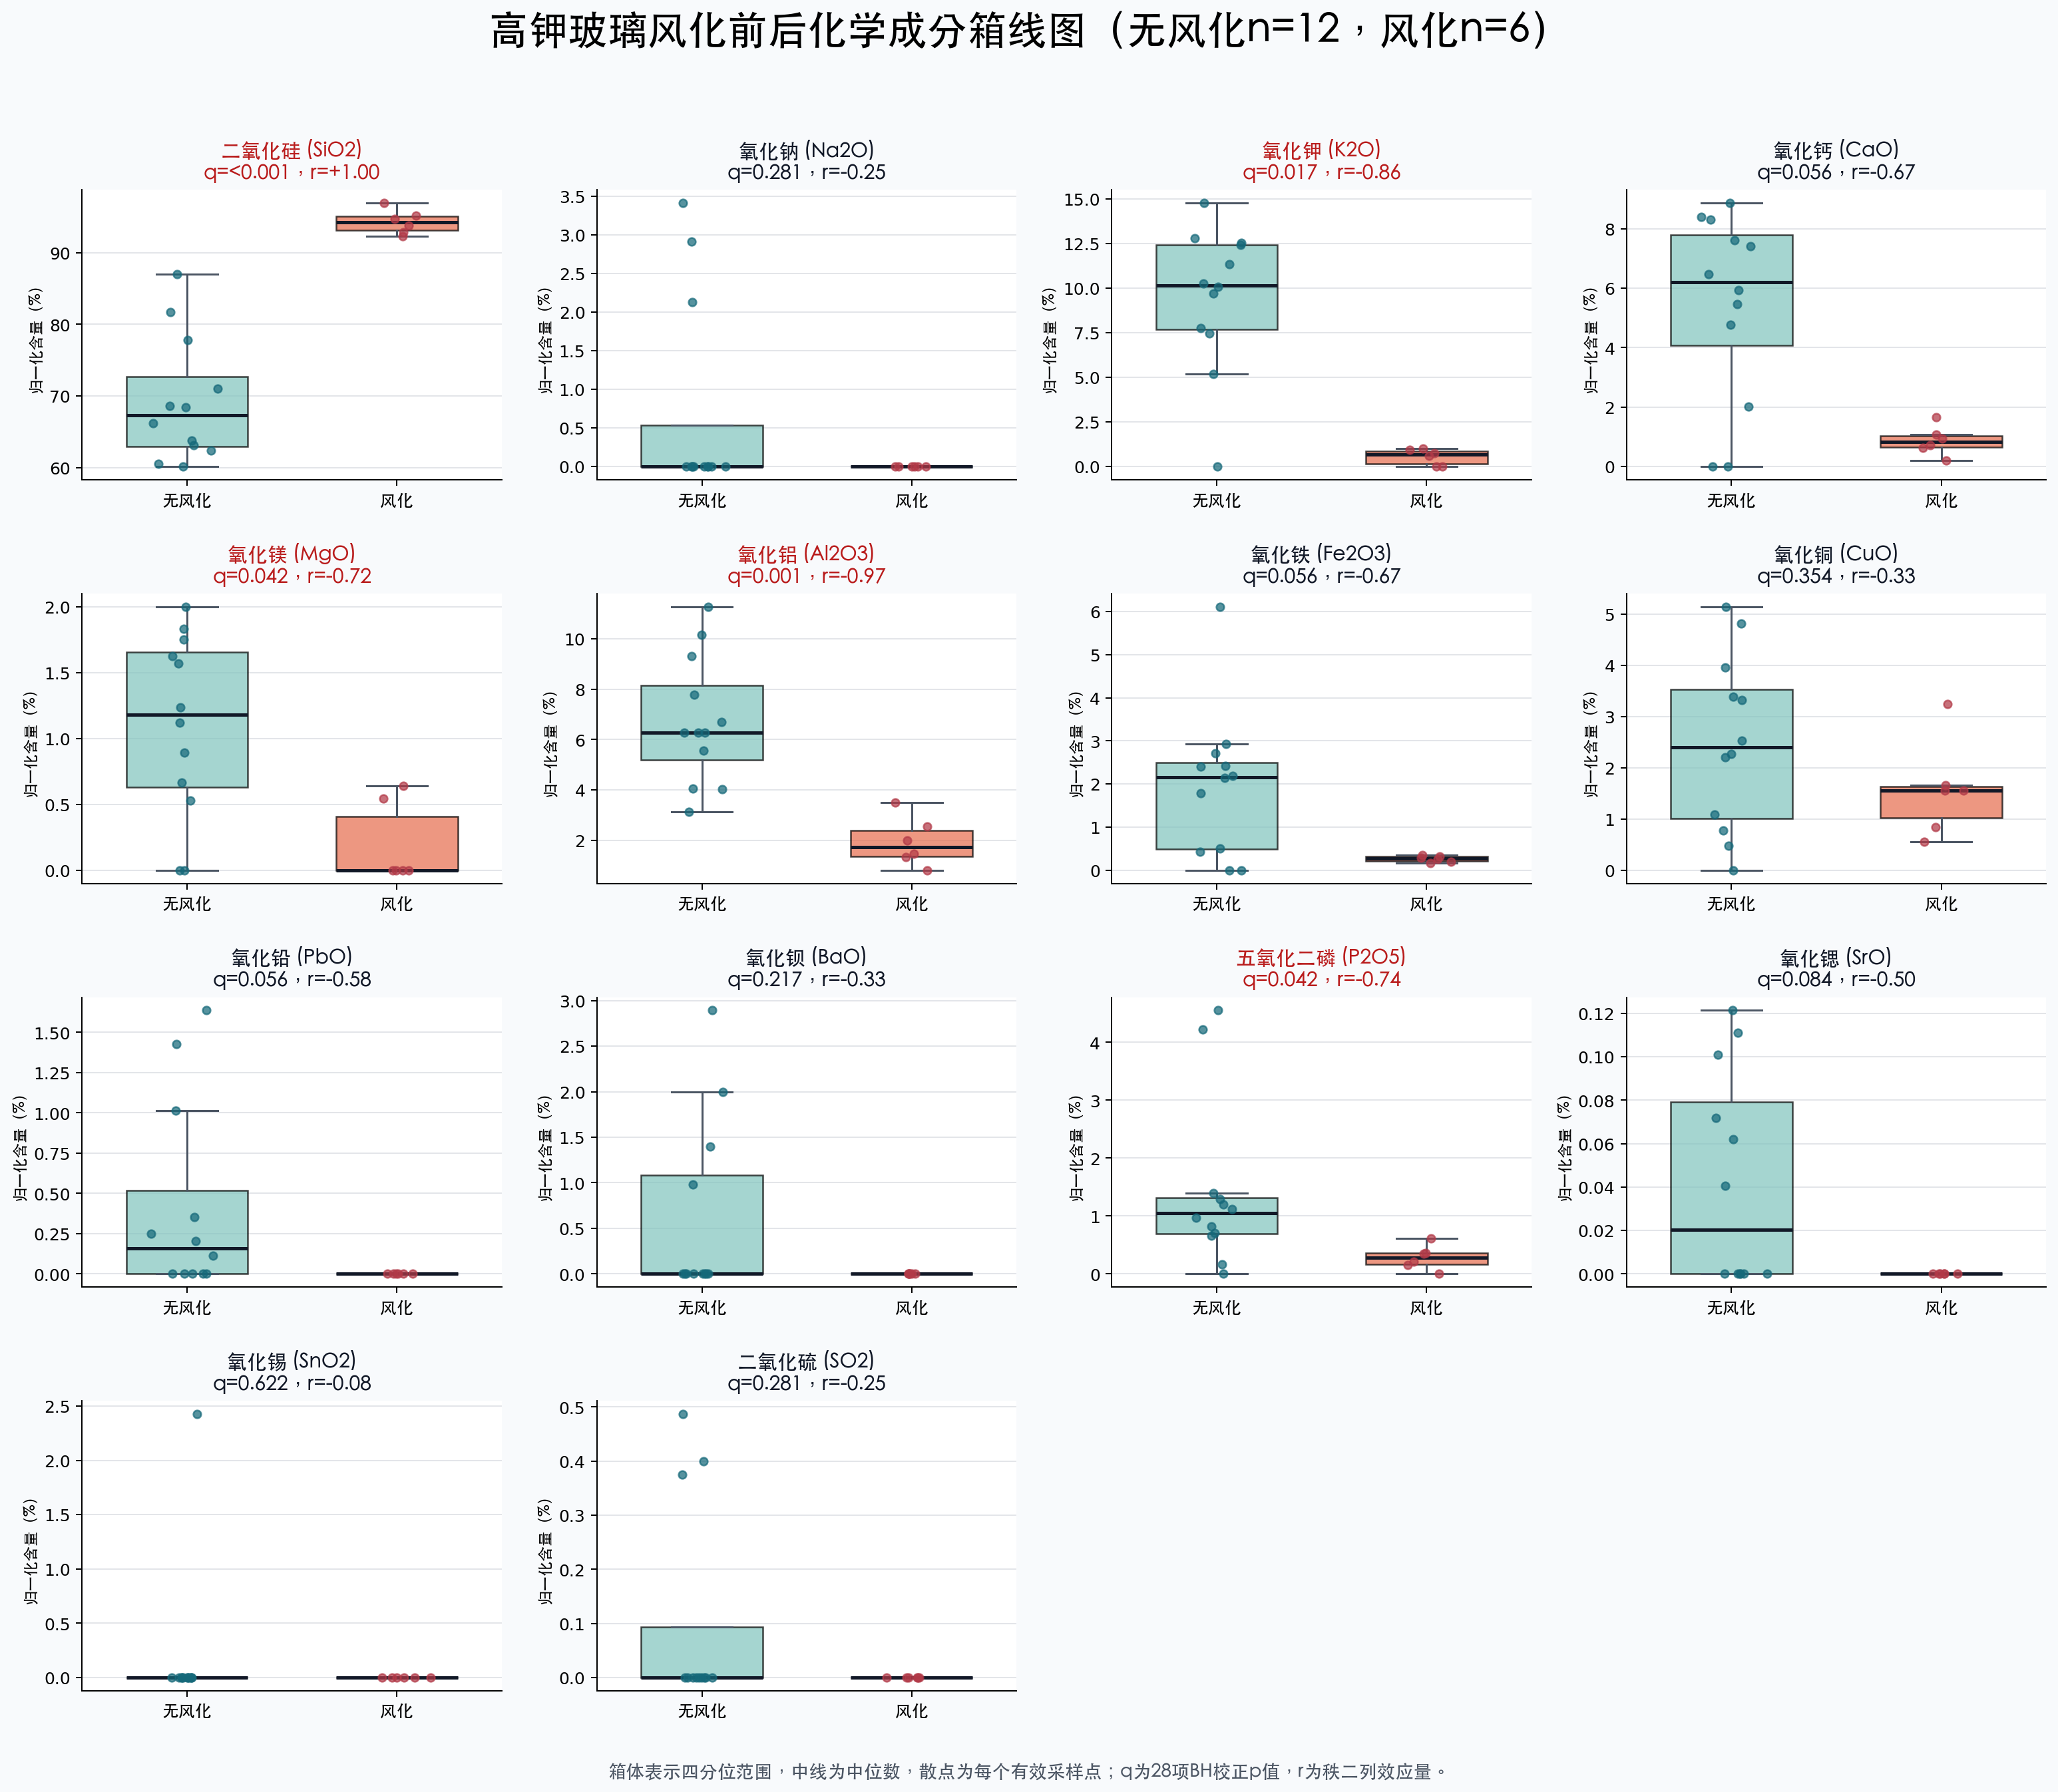
\includegraphics[width=0.96\textwidth]{figures/q1b_high_k_boxplot.png}
    \caption{高钾玻璃风化组与无风化组的化学成分箱线图}
    \label{fig:q1b-high-k}
\end{figure}

铅钡玻璃中，风化组二氧化硅的整体分布明显低于无风化组，而氧化铅、
氧化钙和五氧化二磷的整体分布较高，如图~\ref{fig:q1b-pbba} 所示。
氧化镁、氧化钾和氧化铁等成分的两组箱体及散点重叠较多，其组间差异
相对较弱。

\begin{figure}[H]
    \centering
    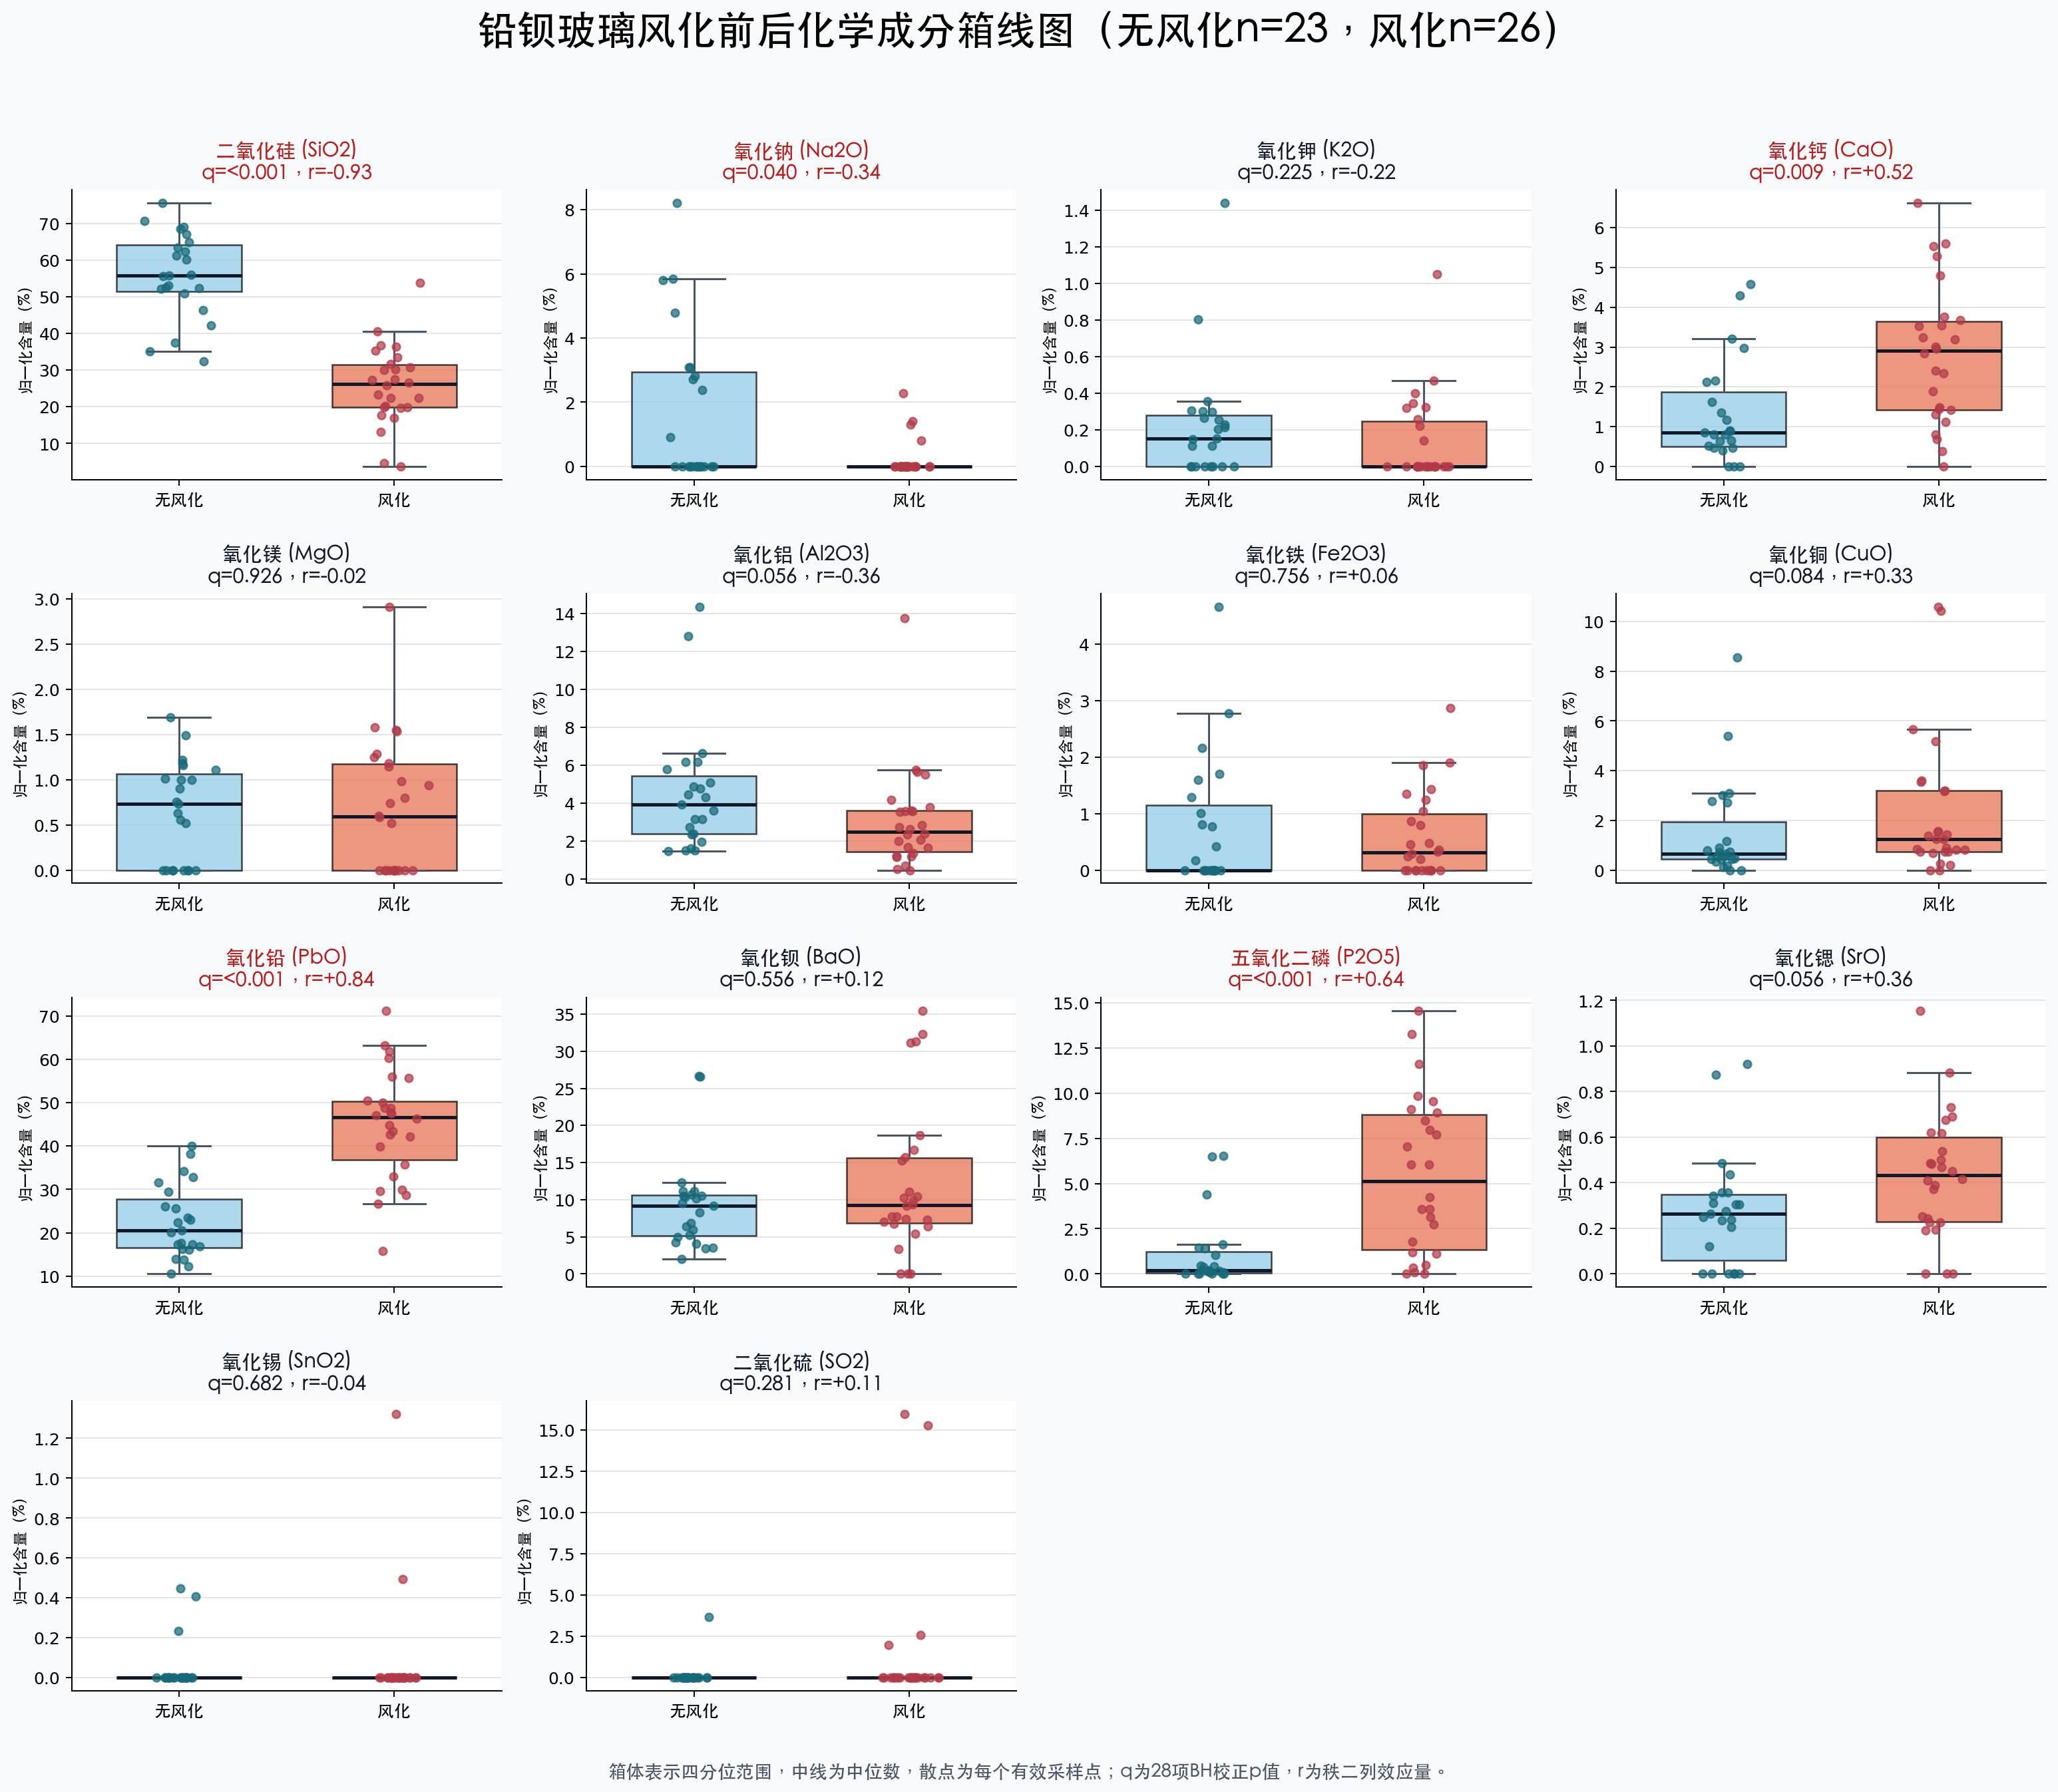
\includegraphics[width=0.96\textwidth]{figures/q1b_pbba_boxplot.png}
    \caption{铅钡玻璃风化组与无风化组的化学成分箱线图}
    \label{fig:q1b-pbba}
\end{figure}

箱线图只能展示样本中的分布差异，不能单独判断这种差异是否足以排除
随机波动。因此，下面结合 Mann--Whitney $U$ 检验、BH 校正和效应量
进行定量判断。

\subsubsection{检验结果与解释}

表~\ref{tab:q1b-high-k} 给出了高钾玻璃经 BH 校正后达到显著水平的
化学成分。风化组二氧化硅相对含量显著较高，且两组样本完全分离
（$q<0.001$，$r_{\mathrm{rb}}=1.00$）；氧化钾、氧化镁、氧化铝和
五氧化二磷相对含量显著较低。氧化钙、氧化铁和氧化铅虽呈下降趋势，
但校正后均为 $q\approx0.056$，未达到 $0.05$ 的显著性标准，故不将其
表述为显著差异。

\begin{table}[H]
    \centering
    \caption{高钾玻璃风化组与无风化组的显著差异成分}
    \label{tab:q1b-high-k}
    \small
    \begin{tabular}{cccccc}
        \toprule
        化学成分 & 风化组方向 & BH 校正 $q$ 值 & $r_{\mathrm{rb}}$ & 效应大小 & 统计结论 \\
        \midrule
        二氧化硅       & 较高 & $<0.001$ & $+1.00$ & 大 & 显著 \\
        氧化钾         & 较低 & $0.017$  & $-0.86$ & 大 & 显著 \\
        氧化镁         & 较低 & $0.042$  & $-0.72$ & 大 & 显著 \\
        氧化铝         & 较低 & $0.001$  & $-0.97$ & 大 & 显著 \\
        五氧化二磷     & 较低 & $0.042$  & $-0.74$ & 大 & 显著 \\
        \bottomrule
    \end{tabular}
\end{table}

铅钡玻璃的显著差异成分如表~\ref{tab:q1b-pbba} 所示。风化组二氧化硅
和氧化钠相对含量显著较低，氧化钙、氧化铅和五氧化二磷相对含量显著较高。
其中，二氧化硅和氧化铅的效应量绝对值最大，说明两组分布的分离最为明显。
氧化铝和氧化锶虽呈一定变化趋势，但其 BH 校正值约为 $0.056$，尚无充分
证据认定其存在显著差异。

\begin{table}[H]
    \centering
    \caption{铅钡玻璃风化组与无风化组的显著差异成分}
    \label{tab:q1b-pbba}
    \small
    \begin{tabular}{cccccc}
        \toprule
        化学成分 & 风化组方向 & BH 校正 $q$ 值 & $r_{\mathrm{rb}}$ & 效应大小 & 统计结论 \\
        \midrule
        二氧化硅       & 较低 & $<0.001$ & $-0.93$ & 大   & 显著 \\
        氧化钠         & 较低 & $0.040$  & $-0.34$ & 中等 & 显著 \\
        氧化钙         & 较高 & $0.009$  & $+0.52$ & 大   & 显著 \\
        氧化铅         & 较高 & $<0.001$ & $+0.84$ & 大   & 显著 \\
        五氧化二磷     & 较高 & $<0.001$ & $+0.64$ & 大   & 显著 \\
        \bottomrule
    \end{tabular}
\end{table}

综上，在现有样本中，两类玻璃呈现不同的风化相关成分特征：高钾玻璃
风化组主要表现为二氧化硅相对含量较高，以及钾、镁、铝、磷相关成分
相对含量较低；铅钡玻璃风化组主要表现为二氧化硅和氧化钠相对含量较低，
而氧化铅、氧化钙和五氧化二磷相对含量较高。由于化学成分属于总和受限
的组成数据，上述“较高”与“较低”均指归一化后的相对含量差异，不应直接
解释为某种元素的绝对增加或流失。此外，部分文物含有多个采样点，本节
结果反映的是采样点层面的统计关联，不能单独作为风化因果效应的证明。



\section{问题二的模型建立与求解}
\subsection{模型建立}
正文内容。

\subsection{求解结果与敏感性分析}
正文内容。

\section{问题三的模型建立与求解}
\subsection{模型建立}
正文内容。

\subsection{模型验证}
说明训练集与验证集的划分、评价指标，以及如何避免数据泄漏。

\subsection{求解结果}
正文内容。

\section{问题四的模型建立与求解}
\subsection{判定模型}
正文内容。

\subsection{评价指标与结果}
给出混淆矩阵、灵敏度、特异度、ROC 或其他与题意相符的指标。

\section{模型评价与推广}
\subsection{模型优点}
\begin{itemize}
  \item 优点一；
  \item 优点二。
\end{itemize}

\subsection{模型局限}
\begin{itemize}
  \item 局限一；
  \item 局限二。
\end{itemize}

\subsection{模型推广}
说明模型可以应用到哪些相似问题，以及需要增加哪些数据。

% ========================= 参考文献 =========================
% 正文中用 \cite{ref1} 引用。以下只是格式示例，提交前替换成真实文献。
\begin{thebibliography}{99}
  \bibitem{ref1} 作者. 文献题名[J]. 期刊名, 年, 卷(期): 起止页码.
  % 使用 AI 时，还应按官方规定列出工具名称、版本/型号、机构和使用日期。
\end{thebibliography}

% ======================= AI 使用声明 ========================
% 必须按真实情况填写，下面两种情况只保留一种。
\section*{AI工具使用声明}
本参赛队使用了AI工具辅助完成部分工作。正式提交前，应在正文相应位置标注AI生成内容，
并在参考文献中列出工具名称、版本或型号、开发机构和使用日期；同时在支撑材料中提交单独的
“AI工具使用详情.pdf”，说明使用环节、关键交互记录、采纳内容和人工修改情况。
% 若完全未使用AI，则把上段改为：本参赛队未使用任何AI工具。

% =========================== 附录 ===========================
\newpage
\begin{appendices}

\section{支撑材料文件列表}
\begin{table}[H]
  \centering
  \caption{支撑材料文件列表}
  \begin{tabularx}{\textwidth}{lX}
    \toprule
    文件名 & 文件说明 \\
    \midrule
    code/problem1.py & 问题一完整可运行程序，请按实际文件修改 \\
    results/result.xlsx & 主要计算结果，请按实际文件修改 \\
    AI工具使用详情.pdf & 使用AI工具时必须提交，请按实际情况填写 \\
    \bottomrule
  \end{tabularx}
\end{table}

\section{源程序}
% 将文件名替换为实际程序；确保程序完整、可运行且与论文结果一致。
% \lstinputlisting[language=Python]{code/problem1.py}

\end{appendices}
\end{document}
